\documentclass{standalone}
\usepackage{mintikz}

\begin{document}
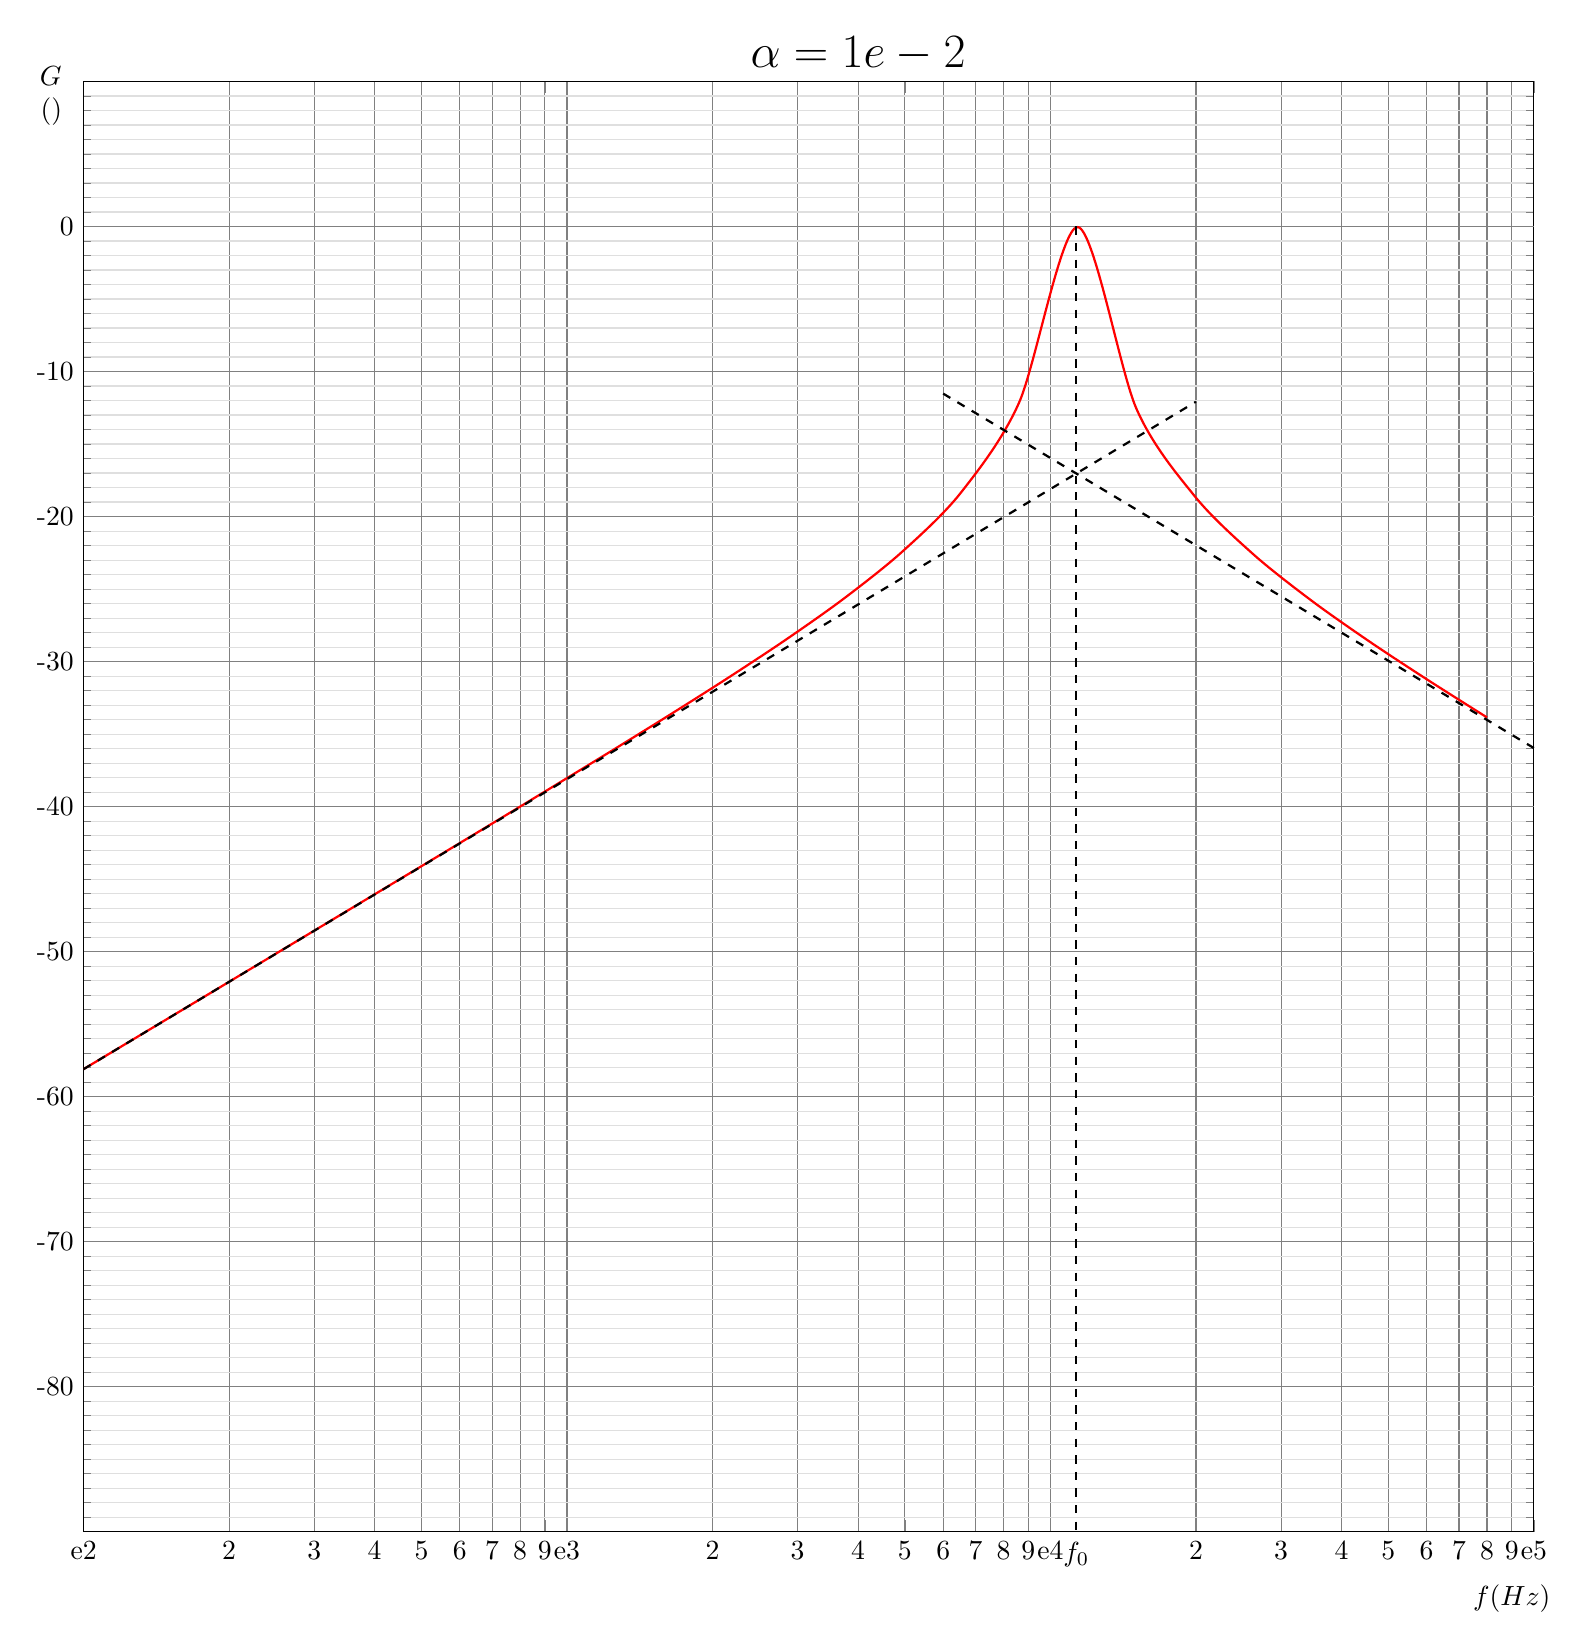
\begin{tikzpicture}
  \def\R{100e3}
  \def\C{1e-9}
	\begin{semilogxaxis}[
			xmin=1e2, xmax=1e5,
			ymin=0, ymax=100,
			ytick={0, 10, ..., 100},
			yticklabels={},
			minor ytick={1, 2, ..., 99},
			extra y ticks={90, 80, ..., 10},
			extra y tick labels={0, -10, ..., -80},
			extra y tick style={grid=none},
			log ticks with fixed point,
			xtick={
					1e2, 2e2, 3e2, 4e2, 5e2, 6e2, 7e2, 8e2, 9e2,
					1e3, 2e3, 3e3, 4e3, 5e3, 6e3, 7e3, 8e3, 9e3,
					1e4, 2e4, 3e4, 4e4, 5e4, 6e4, 7e4, 8e4, 9e4,
					1e5},
			xticklabels={
					\num{e2}, 2, 3, 4, 5, 6, 7, 8, 9,
					\num{e3}, 2, 3, 4, 5, 6, 7, 8, 9,
					\num{e4}, 2, 3, 4, 5, 6, 7, 8, 9,
					\num{e5}},
			width=20cm, height=20cm,
			grid=both,
			minor grid style={gray!25},
			major grid style={black!50},
			clip=false
		]
        \def\a{1e-2}
        \def\Q{sqrt((\a+1)/(2*\a))}
        \def\wo{\Q/(\R*\C)}
        \def\fo{\Q/(2*pi*\R*\C)}
        \def\fop{\fpeval{\fo}}
        \def\Qp{\fpeval{\Q}}
        \addplot[
        domain=1e2:8e4,
        smooth, thick, red]
        {-10*log10(1+\Qp^2*((\x/\fop)-\fop/\x)^2)+90};
        \addplot[
        domain=1e2:2e4,
        smooth, black, dashed, thick]
        {20*log10(\x/\fop)-20*log10(\Qp)+90};
        \addplot[
        domain=6e3:1e5,
        smooth, black, dashed, thick]
        {-20*log10(\x/\fop)-20*log10(\Qp)+90};
		\node[anchor=east, align=center]
		at (axis cs:95,99) {$G_{\dB}$\\$(\si{\dB})$};
		\node[anchor=north]
		at (axis cs:9e4,-3) {$f (\si{Hz})$};
    \draw[dashed, thick]
      (axis cs:\fop,90) --
      (axis cs:\fop,0)
      node[below] {$f_0$};
		\node[anchor=south, align=center]
      at (axis cs:4e3,100) {\LARGE$\boxed{\alpha = \num{\a}}$};
	\end{semilogxaxis}
\end{tikzpicture}
\end{document}
